\documentclass{llncs}

\usepackage{graphicx}
\usepackage{placeins}

\begin{document}

\title{Mobile Alternative of the MoneyBee Project for Financial Forecasting} 

\author{Petar Tomov, Iliyan Zankinski, Maria Barova}

\institute{Institute of Information and Communication Technologies \\
Bulgarian Academy of Sciences \\
acad. Georgi Bonchev Str., block 2, office 514, 1113 Sofia, Bulgaria \\
\email{p.tomov@iit.bas.bg} \\
\texttt{http://www.iict.bas.bg/}}

% Petar Tomov p.tomov@iit.bas.bg 
% Iliyan Zankinski iliyan@hsi.iccs.bas.bg
% Maria Barova m.barova@iit.bas.bg

%----------------------------------------------------------------------------------------
%   Title
%----------------------------------------------------------------------------------------

\maketitle

%----------------------------------------------------------------------------------------
%   Abstract
%----------------------------------------------------------------------------------------

\begin{abstract}
In an attempt to reduce the time for processing of huge volumes of data and algorithms calculations researchers have been addressing the concept of distributed computing for the last couple of decades \cite{balabanov01,balabanov02}. The possibility of utilising the process power of systems in their idle mode has raised yet another much valuable and largely applicable concept, namely donated distributed computing. According to DistributedComputing.Info website, there are hundreds of distributed computing projects in many scientific areas. The most interesting fact, clearly visible in the website, is that there is only one active financial project called MQL5 Cloud Network. Between 2000 and 2010 a German project called MoneyBee was under study. The aim of this project was financial forecasting by artificial neural networks which were trained in a donated distributed computing environment. MoneyBee project was developed and operated by i42 Informations management GmbH company. It was a distributed solution based on a central server and many remote workers. Calculations performed on workers were done during the desktop idle mode while a screensaver was running. In fact, MoneyBee on client machines was the screensaver itself. The goal of the current research is to recreate the ideas used in MoneyBee project on modern mobile devices. Android Live Wallpaper is employed for background calculations executed for training of artificial neural network \cite{keremedchiev01} in the mobile systems idle mode. For the needs of the study two GitHub projects are used - VitoshaTrade and VitDisComp.

\keywords{artificial neural networks, mobile computing, time series forecasting}
\end{abstract}

%----------------------------------------------------------------------------------------
%   Paper
%----------------------------------------------------------------------------------------

\section{Introduction} \label{Introduction}

Financial time series forecasting with the application of artificial neural networks (ANNs) is performed by curve fitting approach \cite{atanasova01}. ANNs are quite common for problems in which unknown mathematical function should be reconstructed only by input/output examples. Generally speaking, ANN is a weighted oriented graph. During the training phase the goal is ANN's weights to be optimized in a way that unknown function to be approximated as accurately as possible. There are many training algorithms. Some of them are exact numerical such as backpropagation of the error \cite{zankinski01}. The others are heuristics. Examples of heuristics are genetic algorithms (GAs) and differential evolution (DE). In many implementations of ANN, weights are not the only subject of optimization. The ANN topology optimization \cite{zankinski02} is another aspect which is very common in the real-life technical solutions. Some evolutionary population based training algorithms are perfect for parallel/distributed implementation because it is easy to split the global population in many local populations \cite{balabanov03}. When donated distributed computing solution is targeted, it is very of high importance how calculations will be divided in parallel processes \cite{balabanov04}. Common difficulties come from the fact that separate calculations will run on separate calculating devices without any synchronization. In GA/DE the problem is represented into the solution space. Each individual in the population is a particular solution. The initial population is established with randomly generated individuals. Afterwards, on each generation some evolutionary operations are applied. Both (GA and DE) are using crossover as general evolutionary calculation. The mutation is a secondary operation, which differs in DE when it is compared to GA. The mutation in DE affects the whole solution \cite{tomov01}, which is not the case in GA, where only a single element of the solution is affected. In case of ANN based forecasting the weights of the ANN are represented as individuals of GA/DE population. This research tries to achieve software solution as MoneyBee project, but implemented on mobile devices. On a central PHP/MySQL based server, global GA/DE population of ANN weights is presented. On the client side, Android background forecasting application is operating local GA/DE populations. This paper is organized as follows: Section \ref{Introduction} introduces the problem; Section \ref{Technical Proposition} presents a mobile donated distributed computing solution; Section \ref{Experiments} gives some experiment details; Section \ref{Conclusions} presents conclusions and some further ideas for research are pointed.

\section{Technical Proposition} \label{Technical Proposition}

In its nature the technical solution is a client-server based software architecture (Fig. \ref{fig01}). A high cost effective choice on the server side is the combination of MySQL, as a relational database management system, and PHP, as a server side scripting language. Both tools are open source and widely available in shared web hosting offerings. Hypertext transfer protocol (HTTP) is one of the most used protocols used in the last two decades for information exchange. The proposed solution uses HTTP in combination with JavaScript object notation (JSON) for structured information exchange. The client side is implemented as Android live wallpaper service. In this way ANN training is performed in the background and it does not affect the regular use of the mobile device. For representation of the ANN structure into device memory, Encog machine learning framework is used in its Java version. The training of ANN is a combination of backpropagation and GA/DE heuristics implemented with Apache commons genetic algorithm library. HTTP communication on the client side is handled with Apache HTTP components library. 

\begin{figure}
  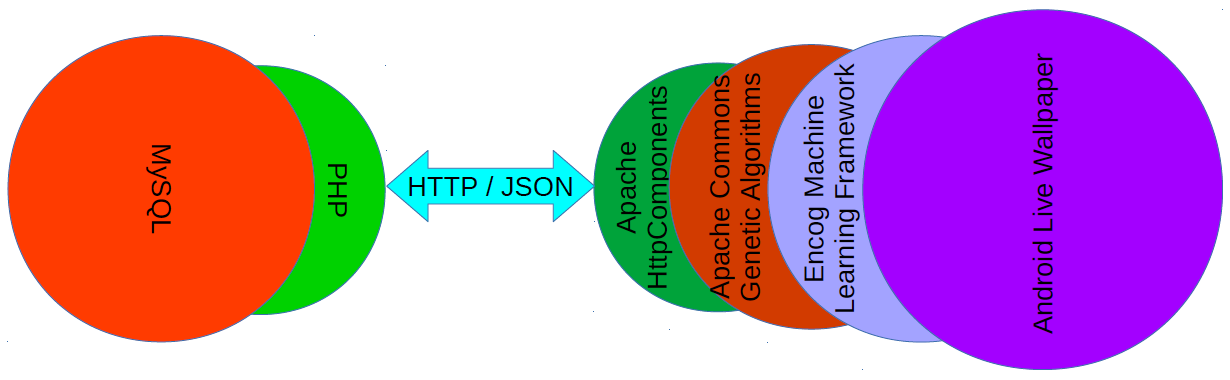
\includegraphics[width=1.0\linewidth]{fig01}
  \caption{Stack of the used technologies.}
  \label{fig01}
\end{figure}
\FloatBarrier

It is very common in distributed computing systems, communications between the server and the clients not to be permanent. When there is a large amount of calculations packed in a single remote job, there is no need of network communication until the job is completed.

\section{Experiments} \label{Experiments}

\begin{figure}
  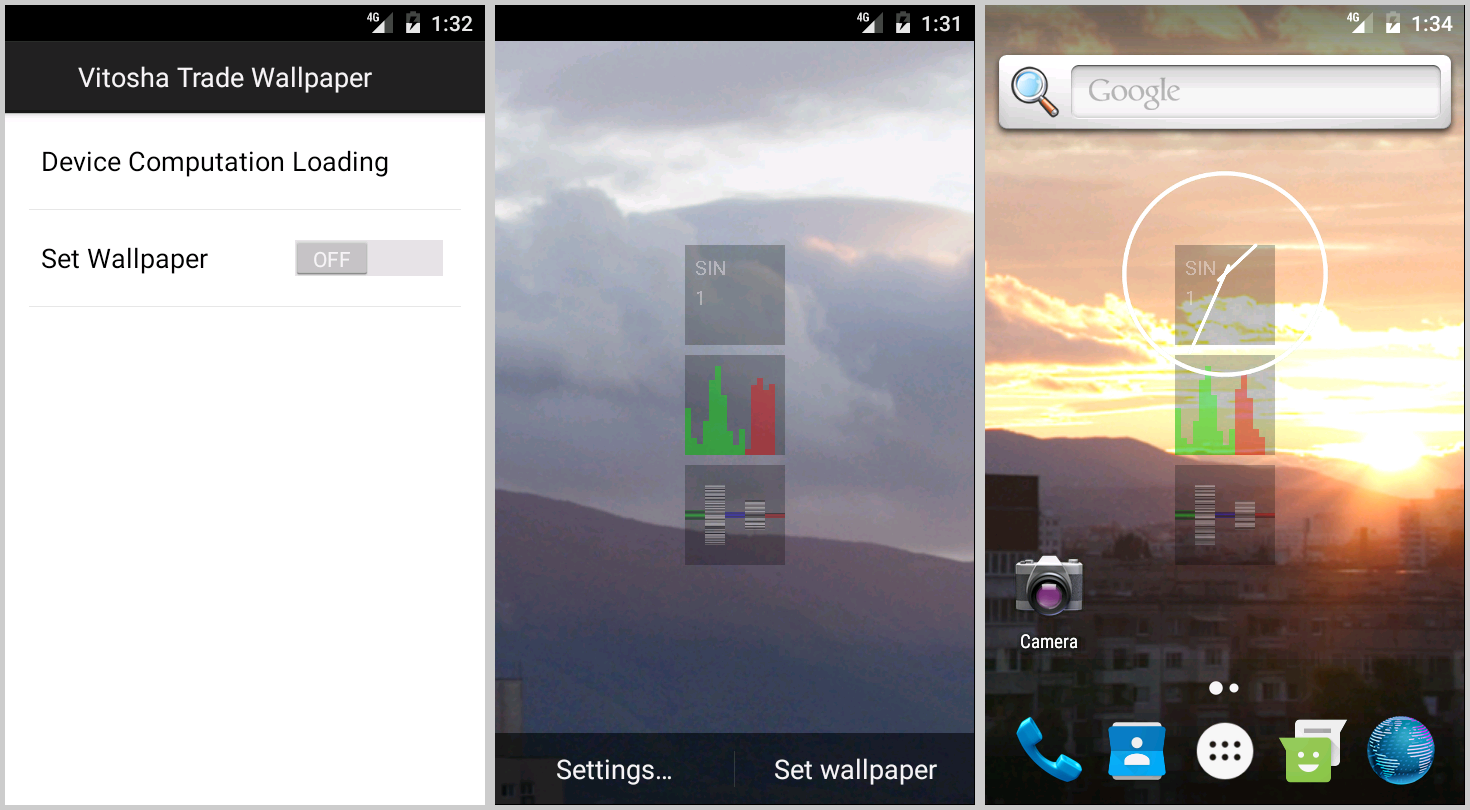
\includegraphics[width=1.0\linewidth]{fig02}
  \caption{Android mobile application (settings screen - left, setup screen - center, running in background - right).}
  \label{fig02}
\end{figure}
\FloatBarrier

Because of the early stage of development, initial system tests are done with generated data (Fig. \ref{fig02}). Further tests are planned with foreign exchange market data (FOREX). At current stage of development the mobile application has settings screen and active wallpaper background calculation mode.  MySQL database is the source of data which are supplied to the remote mobile applications. MySQL database is fed with FOREX data from external MataTrader 4 extension described in \cite{balabanov05}. FOREX data are public and MetaTrader 4 \cite{blackledge01} can provide them in an efficient and accurate way. 

\section{Conclusions} \label{Conclusions}

The success of MoneyBee project (German Federal Ministry of Economy's Multimedia Award Foerderpreis Gruendungswettbewerb Multimedia 1999 in Berlin and the Shortlist 10 Best Ideas at the innovations contest CyberOne 2000 in Stuttgart) can be effectively pursued with the capabilities of the modern mobile devices. With the advanced programming languages and machine learning frameworks, donated distributed computing systems can be developed in a cost effective manner. As further research mobile donated distributed computing can be experimented with the concept of the generalized nets \cite{tashev01,tashev02} or extended Kalman filters \cite{alexandrov01}.

%----------------------------------------------------------------------------------------
%   Acknowledgements
%----------------------------------------------------------------------------------------

\section*{Acknowledgements}

This work was supported by private funding of Velbazhd Software LLC.

%----------------------------------------------------------------------------------------
%   Bibliography
%----------------------------------------------------------------------------------------

\begin{thebibliography}{99}

\bibitem{alexandrov01} Alexandrov, A., Monov, V., \textit{Method for Indoor Localization Optimization of AoA Based Mobile Devices}, Proceedings of 12th Annual Meeting of the Bulgarian Section of SIAM BGSIAM’17, ISSN 1313-3357, 3--3, Sofia, Bulgaria, 2017

\bibitem{atanasova01} Atanasova, T., Barova, M., Balabanov, T., \textit{Use of Neural Models for Analysis of Time Series in Big Data}, Publishing complex of "Vasil Levski" National Military University, ISSN 1314-1937, 193--198, 2016.

\bibitem{balabanov05} Balabanov, T., \textit{Distributed System for Time Series Forecasting with Evolutionary Algorithms and Artificial Neural Networks}, Abstracts of Dissertations of the Institute of Information and Communication Technologies at the Bulgarian Academy of Sciences, vol. 6, e-ISSN 1314-6351, 2017.

\bibitem{balabanov01} Balabanov, T., Genova, K., \textit{Distributed System for Artificial Neural Networks Training Based on Mobile Devices}, Proceedings of the International Conference Automatics and Informatics, Sofia, Bulgaria, Federation of the Scientific Engineering Unions John Atanasoff Society of Automatics and Informatics, ISSN 1313-1850, 49--52, 2016.

\bibitem{balabanov02} Balabanov, T., Keremedchiev, D., Goranov, I., \textit{Web Distributed Computing For Evolutionary Training Of Artificial Neural Networks}, International Conference InfoTech, Varna - St. St. Constantine and Elena resort, Bulgaria, Publishing House of Technical University - Sofia, ISSN 1314-1023, 210--216, 2016.

\bibitem{balabanov03} Balabanov, T., Zankinski, I., Barova, M., \textit{Strategy for Individuals Distribution by Incident Nodes Participation in Star Topology of Distributed Evolutionary Algorithms}, Cybernetics and Information Technologies, Institute of Information and Communication Technologies - BAS, vol. 16, no. 1, ISSN 1311-9702, 80--88, 2016.

\bibitem{balabanov04} Balabanov, T., Zankinski, I., Dobrinkova, N., \textit{Time Series Prediction by Artificial Neural Networks and Differential Evolution in Distributed Environment}. Proceedings of the International Conference on Large-Scale Scientific Computing, Sozopol, Bulgaria, Lecture Notes in Computer Science, Springer, vol. 7116, no. 1, ISBN 978-3-642-29842-4, 198--205, 2011. 

\bibitem{blackledge01} Blackledge, J., Murphy, K., \textit{Forex Trading using MetaTrader 4 with the Fractal Market Hypothesis}, InfoSys 2011: The Third International Conference on Resource Intensive Applications and Services, Venice, Italy, 1--9, 2011.

\bibitem{keremedchiev01} Keremedchiev, D., Barova, M., Tomov, P., \textit{Mobile Application as Distributed Computing System for Artificial Neural Networks Training Used in Perfect Information Games}, Proceedings of the International Scientific Conference, UNITECH’16, Gabrovo, Bulgaria, ISSN 1313-230X, 389--393, 2016.

\bibitem{tashev01} Tashev, T., Marinov, M., Monov, V., Tasheva, R., \textit{Modeling of the MiMa-algorithm for crossbar switch by means of Generalized Nets}, Proceedings of the 2016 IEEE 8th International Conference on Intelligent Systems (IS), Sofia, Bulgaria, ISBN 978-1-5090-1354-8, 593--598, 2016.

\bibitem{tashev02} Tashev, T., Monov, V., \textit{Modeling of the hotspot load traffic for crossbar switch node by means of generalized nets}, Proceedings of the 6-th International IEEE Conference Intelligent Systems IS'12, Sofia, Bulgaria, vol. 2, 187--191, 2012.

\bibitem{tomov01} Tomov, P., Monov, V., \textit{Artificial Neural Networks and Differential Evolution Used for Time Series Forecasting in Distributed Environment}, Proceedings of the International Conference Automatics and Informatics, Sofia, Bulgaria, ISSN 1313-1850, 129--132, 2016.

\bibitem{zankinski01} Zankinski, I., Tomov, P., Balabanov, T., \textit{Alternative Activation Function Derivative in Artificial Neural Networks}, 25th Symposium with International Participation - Control of Energy, Industrial and Ecological Systems, Bankia, Bulgaria, John Atanasoff Union of Automation and Informatics, ISSN 1313-2237, 79--81, 2017.

\bibitem{zankinski02} Zankinski, I., Stoilov, T., \textit{Effect of the Neuron Permutation Problem on Training Artificial Neural Networks with Genetic Algorithms in Distributed Computing}, Proceedings of the 24th International Symposium Management of Energy, Industrial and Environmental Systems, ISSN 1313-2237, Bankya, Bulgaria, 53--55, 2016.

\end{thebibliography}

\end{document}
